\documentclass[11pt,a4paper] {report}

% Aberystwyth MMP Project Report Template for LaTeX
%
% Authors: Neil Taylor (nst@aber.ac.uk) and Dr. Hannah Dee (hmd1@aber.ac.uk) 
%
% This has been adapted from the Leeds Thesis template and the 
% Group Project template for Computer Science in Aberystwyth University.
% 
% All comments and suggestions welcome.
%
% Template designed to be used with pdflatex: it may need alteration to
% run with a different LaTeX engine.
%
% Note - this is offered as a starting point for your work. You are not 
% required to use this template and can choose to create your own document 
% without it.

% This template is suitable for students with an engineering-style project, 
% which will be most students in the department. If your project is a research-oriented 
% project, look at the alternative template.

% To build document on the unix command line, run four commands:
 
%pdflatex mmp-report
%bibtex mmp-report
%pdflatex mmp-report
%pdflatex mmp-report

% you will end up with abd15_mmp-report.pdf. Before submitting, add your user ID as a prefix,
% e.g. abc01-abd15_mmp-report.pdf
\usepackage{StylesAndReferences/mmp-report-style}

% the following packages are used for citations - You only need to include one. 
%
% Use the cite package if you are using the numeric style (e.g. IEEEannot). 
% Use the natbib package if you are using the author-date style (e.g. authordate2annot). 
% Only use one of these and comment out or remove the other one. 
\usepackage{cite}
%\usepackage{natbib}

%%%% Title and Section Colours %%%%
% Modify these values to change the colours used for title, sections and subsections.
% Each value is a range of 0-255 in RGB colourspace.
% Idea courtesy of discussion at 
% https://www.overleaf.com/learn/latex/Using_colours_in_LaTeX
% and
% https://tex.stackexchange.com/questions/75667/change-colour-on-chapter-section-headings-lyx
% 
% If you prefer to have black headers, then comment out the following lines
\definecolor{mmpTitle}{RGB}{10, 85, 145}
\definecolor{mmpSection}{RGB}{10,85,155}
\definecolor{mmpSubsection}{RGB}{79,129,189}

\chapterfont{\color{mmpTitle}}  % sets colour of chapters
\sectionfont{\color{mmpSection}}  % sets colour of sections 
\subsectionfont{\color{mmpSubsection}} % sets colour subsections
\subsubsectionfont{\color{mmpSubsection}} % sets colour subsections

%%%% end of Title and Section Colours %%%%


%%%% Report Type %%%%
%% comment/uncomment depending on the type of report you want to generate
\reporttype{Engineering}
%\reporttype{Research}
%%%% end of Report Type %%%%


\begin{document}

%TC:ignore

% all of the include directives below refer to tex files
% so %TC:ignore 

\title{Satellite Imagery Land use classification using Machine Learning}

% Your name
\author{Abdullah Durrani}

% Your email 
\authoremail{abd15@aber.ac.uk}

\degreeschemecode{GH76} %e.g. G400
\degreeschemetitle{Artificial Intelligence and Robotics} % e.g. Computer Science
\degreetype{BSc}

\modulecode{CS39440} % i.e. CS39440, CC39440, CS39620
\moduletitle{Major Project} % i.e. Major Project or Minor Project

\date{23rd April 2024} % i.e. the date of the current version of your report

\status{release} % Use draft until you create the release version. Then, change this to Release.
\version{1.0}

% The title and name of your supervisor.
\supervisor{Dr/Prof. Tossapon Boongoen}

%The email for your supervisor. 
\supervisoremail{tob45@aber.ac.uk}

\maketitle

%TC:endignore
 includes cover.tex - to change the content,
% edit the tex file

\raggedright
\pagenumbering{roman}

% This is the front page
%TC:ignore 

\title{Satellite Imagery Land use classification using Machine Learning}

% Your name
\author{Abdullah Durrani}

% Your email 
\authoremail{abd15@aber.ac.uk}

\degreeschemecode{GH76} %e.g. G400
\degreeschemetitle{Artificial Intelligence and Robotics} % e.g. Computer Science
\degreetype{BSc}

\modulecode{CS39440} % i.e. CS39440, CC39440, CS39620
\moduletitle{Major Project} % i.e. Major Project or Minor Project

\date{23rd April 2024} % i.e. the date of the current version of your report

\status{release} % Use draft until you create the release version. Then, change this to Release.
\version{1.0}

% The title and name of your supervisor.
\supervisor{Dr/Prof. Tossapon Boongoen}

%The email for your supervisor. 
\supervisoremail{tob45@aber.ac.uk}

\maketitle

%TC:endignore
                        

% Set up page numbering
\pagestyle{empty}

% declarations of originality 
\thispagestyle{empty}

%TC:ignore

%%%
%%% You must sign the declaration of originality. 
%%%
%%% You are submitting this electronically. Therefore, to sign, you 
%%% type your name and date to replace the .... characters. 
%%%
\section*{\centering Declaration of originality}

I confirm that:

\begin{itemize}
\item{This submission is my own work, except where 
clearly indicated.}

\item{I understand that there are severe penalties for Unacceptable Academic Practice, which can lead to loss of marks or even the withholding of a degree.}
 
\item{I have read the regulations on Unacceptable Academic Practice from the University's Academic Registry (AR) and the relevant sections of the current Student Handbook of the Department of Computer Science.}
 
\item{In submitting this work I understand and agree to abide by the University's regulations governing these issues.}
\end{itemize}

\vspace{2em}
Name ............................................................  \\

\vspace{1em}
Date ............................................................ \\

%%% 
%%% We would like to make a selection of final reports available to students that take 
%%% this module in future years. To enable us to do this, we require your consent. You 
%%% are not required that you do this, but if you do give your consent, then we will have 
%%% the option to select yours as one of a number of reports as examples for other 
%%% students. If you would like to give your consent, then please include the following 
%%% text and type your name and date to replace the .... characters. 
%%% 
%%% If you do not wish to give your consent, please remove this from your report. 
%%%
\vspace{1em}
\section*{\centering Consent to share this work}

By including my name below, I hereby agree to this project's report and technical work being made available to other students and academic staff of the Aberystwyth Computer Science Department.  

\vspace{2em}
Name ............................................................  \\

\vspace{1em}
Date ............................................................ \\

%TC:endignore

               

\thispagestyle{empty}

%TC:ignore

\section*{\centering Acknowledgements}

I would like to thank my supervisor Prof. Tossapon Boongoen for all his help in supporting me through this project I could
not have gotten to here writing this report without Your encorigment to always do my best.
%TC:endignore % Acknowledgements

\thispagestyle{empty}

%TC:ignore
\section*{\centering Abstract}

This report states the process utilized in developing a python application that employs
the K-means clustering algorithm for the classification of satellite imagery.
The primary objective of this project was to simplify and enhance the usage of satellite data across various sectors
by providing a user-friendly tool for image analysis.

The application incorporates a single classifier which can be expanded to include other unsupervised classifiers as well as supervised ones
, but the K-means algorithm, which is renowned for its efficiency in segmenting images into clusters based on pixel similarity.
This method is particularly advantageous for categorizing land use and identifying patterns or changes in satellite images.

Research was conducted to ensure the optimal implementation of the K-means algorithm, with studies indicating its effectiveness
in handling large datasets and its robustness in producing significant clusters that are meaningful in the context of satellite imagery.

Designed to be intuitive, the application allows users of varying technical expertise to engage with satellite data analysis.
The system facilitates real-time processing of images, providing immediate feedback and results of the effectiveness of the Kmeans implementation,
and allows for the user to compare images overtime visually highlighting differences.
which are crucial for timely decision-making in areas such as environmental monitoring and urban planning among other areas.

%TC:endignore                 % Abstract

\pagenumbering{roman}
\pagestyle{fancy}
\fancyhead{}
\fancyfoot[C]{\thepage}
\renewcommand{\headrulewidth}{0 pt}
\renewcommand{\chaptermark}[1]{\markboth{#1}{}}

\tableofcontents   
\newpage
\listoffigures % comment out this line if you don't have any figures / graphics
\newpage 
\listoftables % comment out this line if you don't have any tables
\newpage

% Set up page numbering
\pagenumbering{arabic}

\setchapterheaderfooter

%TC:endignore

% include the chapters
\chapter{Background \& Objectives}


\section{Background}

\section{Analysis}

\section{Process}

\chapter{Experimentation}\label{ch:experimentation}


\section{K-Means clustering}\label{sec:k-means-clustering}

This section is about how the Kmeans clustering algorithm works mathematically.
As it is important that we learn how the Classifier functions so that we can understand how Clustering occurs,
what the processes are, and how we can manipulate it to get the best possible results.
The steps are as follows:

\begin{itemize}
    \item \textbf{Initialization:}
    \textit{The first step in k means clustering involves selecting K initial centroids, where k is the number of clusters
    you want to identify in the dataset.
    The centroids can be randomly selected from the datapoints, or you can provide a heuristic or specific strategy
    on which they are chosen to enhance the quality and or speed of convergence.}
    \item \textbf{ Assignment step}
    \textit{In this step each data point in the dataset is assigned to the nearest centroid.
    the nearest is determined by the euclidian distance between the data point and the centroid this is mathematically determined by
    \[
        C_i = \{ x_p : \|x_p - m_i\| \leq \|x_p - m_j\| \, \forall j, 1 \leq j \leq k \}
    \]}
    \textit{where $C_i$ is the set of data points assigned to cluster $i$, $x_p$ is a data point, and $m_i$ is the centroid
    of cluster $i$. This means each data point $x_p$ is assigned to cluster $i$ if the distance from $x_p$ to $m_i$ is the smallest
    among all centroids.}
    \item \textbf{Update Step}
    \textit{Once all data points have been assigned to clusters, the centroids need to be recalculated.
    This is done by taking the mean of all points assigned to each cluster—the position of the centroid of each cluster is updated
    to the mean position of all points belonging to that cluster. The formula for updating the centroid of each cluster is:
    \[
        m_i = \frac{1}{|C_i|} \sum_{x \in C_i} x
    \]}
    \textit{where $|C_i|$ is the number of data points in cluster $i$, and $\sum_{x \in C_i}$ is the sum of all data points
    in cluste $i$}
    \item \textbf{Iteration}
    \textit{ In this step steps 2 and 3 are repeqted iterativly until the centroilds stop moving significantly, this means
    that the cluster is now stabilized and the algorithm has converged, the number of iterations has been spent. This allows
    the cluster assignmenst and centeroid positions to reflect the data accurately.}
    \item \textbf{Convergence}
    \textit{The algorithm has converged when the centroids have stabilized and or alternatively when the assignment of points to clusters
    longer change }
\end{itemize}

\section{Metrics Used}\label{sec:metrics-used}

When Employing Clustering algorithms such as K-means, assessing the quality of the algorithm is important as it validates
the effectiveness of the analysis.
Because of this, I use three crucial metrics to evaluate the K-means algorithm Silhouette score, Inertia and DBI(Davies-Bouldin Index)

\subsection{Silhouette Score}\label{subsec:silhouette-score}

The Silhouette Score is a measure of how similar an object is to its own cluster compared to other clusters.
The score is calculated for each data point and can range from -1 to +1, where a high value indicates that the object is
well-matched to its own cluster and poorly matched to neighboring clusters
Mathematically its definition is:
\[
    s(i) = \frac{b(i) - a(i)}{\max(a(i), b(i))}
\]
    $a(i)$ is the mean distance between $i$ and all other data points in the same cluster.

    This measures how well it $i$ is assigned to its cluster (the smaller, the better).

    $b(i)$ is the minimum mean distance from ii to all points in any other cluster, of which $i$ is not a member.

    This measures how poorly $i$ is matched to its neighboring cluster (the larger, the better).

The overall Silhouette Score for the dataset is the mean Silhouette Score of all individual points.
    This score provides a succinct measurement of how appropriately the data has been clustered.

\subsection{Inertia}\label{subsec:inertia}

Inertia, also known as the within-cluster sum of squares, measures the compactness of the clusters, which ideally should be as small as possible .
It is calculated by summing the squared distances between each data point and its nearest centroid.
Mathematically its definition is:
\[
   W(C) = \sum_{i=1}^k \sum_{x \in C_i} \|x - \mu_i\|^2
\]



$C_i$ is the set of all points in cluster $i$,

$mu_i$ is the centeroid of cluster $i$

Outer Sum: $\sum{i = 1}^k$ iterates over each cluster from 1 to $k$.

Inner Sum: $\sum{x \in C_i}$ sums over all points $x$ within each cluster $C_i$.

$ \|x - \mu_i\|^2$ computes the squared Euclidean distance between a point $x$ and the cluster centroid $mu_i$,
which is the norm squared of the vector difference.

$k$ is the number of clusters

\subsection{Davies-Bouldin Index (DBI)}\label{subsec:davies-bouldin-index-(dbi)}

The DBI is Defined as the Average similarity measure of each cluster with its most similar cluster, where similarity is the ration of within cluster distances
to between cluster differences.
The Goal is to minimize the DBI, as a lower DBI score indicates a better clustering division.
It has no dependency on the Shape or Density of the Cluster, It is easy to compute, and it is a Simple interpretation as it directly
quantifies the trade-off between the compactness of clusters and their separation.
The Mathematical definition for it is:
\[
    DBI = \frac{1}{k} \sum_{i=1}^k \max_{i \neq j} R(i,j)
\]
where $k$ is the number of clusters, and $R(i,j)$ is the similarity measure between clusters $i$ and $j$ where $R(i,j)$
is defined as $R(i,j) = \frac{s_i+s_i}{d_{ij}}$

$s_i$ is the average distance to all points in cluster $i$ to the centroid of cluster $i$ (intra-cluster distance)

$d_{ij}$ is the distance between the centroids of clusters $i$ and $j$ (inter-cluster distance)

$s_j$ is similarly the average intra-cluster distance for cluster $j$.

\section{Analysis of Clustering Metrics: Determining the Optimal Number of Clusters for the Al Dhannah Dataset}\label{sec:analysis-of-clustering-metrics:-determining-the-optimal-number-of-clusters-for-the-al-dhannah-dataset}

The selection of the optimal number of clusters (k) in K-means clustering is crucial for achieving the best possible grouping of data points.
We can analyze this by reviewing graphs of the Average Inertia for Different k, Average Silhouette Scores for Different k,
and a combined plot of Silhouette Score vs.Inertia so that we can find the best K for the Al Dhannah City dataset as each
dataset will have a different best K\@.

\subsection{Average Inertia for different K}\label{subsec:average-inertia-for-different-k}



As illustrated in Figure\ref{fig:1}, As we can see from the Graph, there is a sharp decline in inertia as the number of Clusters increases from 2 to around 5 followed
by a more gradual decrease.
The Lower the Inertia value, the more Compact the Clusters meaning higher quality clusters.

We can apply the elbow rule here which states that the optimal K is where the inertia curve begins to flatten in this graph the
curve begins to flatten around K=4.
this suggests that increasing the number of clusters beyond this point results in Diminishing results


\subsection{Averge Silhouette Scores for Different K}\label{subsec:averge-silhouette-scores-for-different-k}



As illustrated in Figure\ref{fig:2}, The Average Silhouette Score graph presents a different perspective, highlighting the average silhouette score of clusters as k varies.
The silhouette score measures how similar an object is to its own cluster compared to other clusters, with higher values generally indicating more appropriate clustering.

The graph shows the highest silhouette score at k=2, which then declines steadily as more clusters are added.
This indicates that at k=2, the clusters are more distinct and well-separated compared to higher values of k.

\subsection{Silhouette Score vs. Inertia}\label{subsec:silhouette-score-vs.-inertia}



As illustrated in Figure\ref{fig:3}, The combined graph Plots these scores against each other for the value of k this visual representation helps us see the
trade-off between Inertia and the Silhouette score.
If K is high in this dataset, inertia is low, so K = 2 is too much in favor of the Silhouette Score, the Clusters are separate, but the
clusters are not as dense as they should be.
K = 4, on the other hand, is perfect as The silhouette Score is not as good as K = 3 and the inertia is not as good as K = 5.

Using insights from Both previous graphs.
We can determine that K = 4 is the most balanced choice for the Current Dataset as
it provides a compromise between having distinct clusters and ensuring that the clusters are compact enough\cite{studentResults2022}.
This is suggested by the elbow in the inertia graph and relatively good silhouette scores for K = 4 in the silhouette score graph.


\chapter{Design and Implementation}\label{ch:design-and-implementation}

As we are following the Feature Driven Development methodology
which was discussed in section~\ref{subsec:feature-driven-development-(fdd)-overview} the Design,
Implementation, and Testing Chapters of the report have been merged
For each iteration of the Project a section has been created to report on the progress made for each iteration

\section{ Iteration 0}\label{sec:iteration-0}

This iteration was spent researching and creating a design prototype as well as figuring out the feature list of the
application.
This iteration was also spent researching where to collect data

\subsection{Initial Design}\label{subsec:initial-design}

The initial design of the Satellite Image Classification System was conceived to provide a robust,
user-friendly platform
for the analysis and classification of satellite imagery using machine learning techniques.
The design focused on creating a modular, scalable,
and intuitive application that could be easily adapted to meet the diverse needs
of users ranging from environmental scientists to urban planners.

The Initial design would be object orientated, and did not currently have a specific Machine learning Model in mind for
the application there wer 4 different models in line for the spot Random Forrest, CAST(Decision tree), CNNs and K-means clustering
Initially the Criteria for Model selection was Performance, Scalability and Accuracy.

Below is an initial Architecture for what
the Program should have been able to do it consists of 3 Layers A User interface Layer,
Data processing layer and a machine learning Layer

\begin{itemize}
    \item \textbf{User interface Layer}
    \item  \begin{itemize}
               \item \textbf{Functionality}
               \textit{The UI layer, provides the primary interaction point for users.
               It handles tasks like loading images, initiating the classification process, displaying results, and enabling
               comparative analysis of images.}
               \item \textbf{Technology}
               \textit{It utilizes the Tkinter library, a standard GUI toolkit in Python, which supports building desktop applications
               with graphical elements like buttons, canvases, and dialog boxes.}
            \end{itemize}
    \item \textbf{Data Processing Layer}
    \item  \begin{itemize}
               \item \textbf{Functionality}
               \textit{This layer, is responsible for preparing the image data for analysis.
               This includes preprocessing tasks such as resizing, and normalizing the pixel data of the image,
                   and making sure the images are in the optimal format for clustering.}
               \item \textbf{Output}
               \textit{It outputs the Image as Usable data for the machine Learning layer}
           \end{itemize}
    \item \textbf{Machine Learning layer}
    \item   \begin{itemize}
               \item \textbf{Functionality}
               \textit{he core analytical capabilities of the system are handled by the machine learnning algorithm to the processed image data,
                   classifing  the images into distinct land uses based on their features.}
               \item \textbf{Features}
               \textit{It calculates key metrics after classification testing for accuracy, and classifier Performance}
            \end{itemize}
\end{itemize}


\subsection{Use case Diagram}\label{subsec:use-case-diagram}

The use case diagram provided in Figure\ref{fig:5} offers a visual representation of the interactions between the user and the Satellite Image Classification System.
It outlines the key functionalities and flow of operations within the system,
highlighting how users engage with the software to achieve their objectives

\subsection{Activity Diagram}\label{subsec:activity-diagram}

This activity diagram provided in figure\ref{fig:6}shows how the user will interact with the program and what the program should be doing depending on what the user does


\subsection{Data Collection}\label{subsec:data-collection}

Data for the Project was collected is collected from rom the Copernicus web browser, a part of the Copernicus Earth Observation Program.
This program provides a comprehensive suite of satellite data encompassing a wide range of environmental and security applications,
making it an invaluable resource for our system.
Specifically, we took data From the Sentinel 2a satellite.
We chose JPG over the TIFF and PNG because of three main reasons:

\begin{itemize}
    \item \textbf{Accessibility}
    \textit{Jpg is one of the most common image formats on the internet, it's highly compatible and support across various platforms and devices. 
    This makes JPG an ideal choice for ensuring that the application is accessible to a broad audience }
    \item \textbf{Ease of use}
    \textit{By using Jpg, the system simplifies the user experience, as most users are already familiar with handling and viewing JPG files.
    This familiarity eliminates potential barriers to entry}
    \item \textbf{Memory Constraints}
    \textit{ PG images offer the advantage of compression, which reduces file sizes significantly.
    This compression enables more efficient storage and faster transmission of images,
        which is particularly beneficial when dealing with large datasets typical in satellite imagery}
\end{itemize}

\subsection{Feature List}\label{subsec:feature-list}

A feature List \ref{tab:1} for the required features in the Land Use Classification application.
the features are designed to provide a comprehensive toolset for users, ensuring not only the functionality to process and classify
images but also to manage resources effectively


\section{Iteration 2}\label{sec:iteration-2}

During the second iteration of developing the land use classifier project,
the primary focus was on implementing the crucial image loading functionality.
This feature enables users to upload their satellite imagery into the system,
setting the stage for subsequent processing and analysis of the image

\subsection{Development phase}\label{subsec:development-phase}

during the development phase of iteration 2, We developed image processing functions using the pillow and open CV libraries.
These libraries provided the necessary tools for checking image integrity and performing necessary transformations such as format,
conversion and resizing useful for machine learning applications

we did a series of \ref{tab:2}tests which succeeded all of them except one,
Which was a semi-fail because The corrupted image in the test was not detected by the program
but it was also not used by the program and when the program you tried to use it,
the program did not crash but sent an internal error so it was a semi-fail
After implementing the image loader for the project.

\section{Iteration 3}\label{sec:iteration-3}

During the third iteration of the program, the primary focus was on getting the next two features from the feature list up and running.
These were the image viewer and the classification configure settings.
Both of these culminated in The creation of the main window class.
This was the main way for the user to interact with the program from this main window.
They could view the images, load their own images onto the program.
enter k for the K-means classifier which we had chosen by this point to be the classifier that we would develop next.
and pressing the start classification button which didn't really do anything at this point it was just more for show

\subsection{Development Phase}\label{subsec:development-phase2}

Integration of key features: image viewer development purpose was to allow users to visually inspect and manage the satellite images they uploaded functionality.
The image viewer was designed to display images within the application Interface.
The Classification configuration settings purpose was to provide users with the ability to configure the parameters
for the k-means clustering algorithm which was selected as the classification technique.
users could enter the number of clusters for the k means algorithm.
The setting is crucial for turning the classification process to meet the specific needs of the user,
such as distinguishing between different types of geographical features or land uses.
The main window class now acts as a central hub for user interactions.
Within the applications design, the main window class was developed to integrate various functionalities,
including image loading, viewing and configuration settings into a single, coherent interface.
This design approach ensures that users have a centralised and intuitive interface from which they can control all major aspects of the application


\section{Iteration 4}\label{sec:iteration-4}

Iteration 4 of the land use classification system marked a pivotal development phase, introducing the core ImageProcessor and KProcessor classes.
The ImageProcessor class handles initial image manipulations, resizing images for uniformity, flattening them into arrays, normalizing data,
and reshaping these into 3D arrays suitable for clustering.
These pre-processed images are then passed to the KProcessor class,
which applies K-means clustering, calculates key metrics like silhouette score, inertia, and Davies-Bouldin Index (DBI),
and performs cluster remapping to ensure color consistency across visual outputs.
This remapping involves sorting the indices of cluster centers by the sum of their coordinates and creating a new,
orderly mapping from original to sorted indices.
This sophisticated data processing and clustering functionality,
integrated back into the main window class,
significantly enhances the system’s ability to provide robust image classification and analysis,
making this iteration a substantial leap forward in the system's development.

Manual Testing on this Iteration was done in \ref{ch:experimentation}

\subsection{the Development Phase}\label{subsec:development-phase3}

Iteration 4 marked, a significant advancement in the development of the land use classifier system with the introduction of the km processing class and the image processor class.
This phase represented the core of the project functionality where the primary processing and clustering operations were implemented.
Overview of new classes and functionalities:
The image processor class's purpose is to prepare the raw satellite images for clustering by performing a series of pre-processing steps.
like image resizing the image to ensure uniformity across all images.
It Flattens the image and normalizes the values of the image.
Reshapes the flattened array into a 3D array appropriate for the clustering process.
The km processing class purpose handles the clustering of pre-processed image data using the k means algorithm and calculates relevant clustering metrics.
Functionality: The k means algorithm applies clustering to segment the image data into a specified number of clusters.
metric calculation computes key performance metrics like silhouette score, inertia and the Davies bolden index or DBI to assess the quality of the clustering cluster.
Remapping adjust the labelling of clusters to ensure consistency in colour mapping across different plots.
Enhancing the visual coherence of cluster representations and is important for the last feature which is difference maps
The processed data, along with the clustering results and metrics, are then passed back to the Main Window class.
This integration allows users to interact dynamically with the processed images, view clustering results,
and analyze the performance metrics directly through a user-friendly interface.




\section{Iteration 5}\label{sec:iteration-5}

Iteration 5 of the land use classification focused on the development of the display results page a used the clusters
that had been taken from the km processing object and used matplotlib to clot the cluster.
Be it singular or plural with the metrics that had been calculated for that specific plot,
so that would be the silhouette score inertia and Davies Bowden index



\subsection{the Development Phase}\label{subsec:development-phase4}

iteration 5 of the land use classifier system was centred around the development of the display results page which plays a crucial role in visualising the outcomes of the land use classification process this phase leveraged the class clustering data processed by the km processing class from the previous iterations utilising the popular python library matplotlib to create
informative and interactive visualisations of the clustered satellite images, key features and functionalities developed cluster visualisation.
The system now integrates functionality to display the clustered images directly on the results page when showing a single cluster or multiple clusters.
The visualisations are designed to be clear and distinguishable enhancing the user's ability to interpret the data integration of matrix alongside the visual representations key clustering metrics such as the silhouette score inertia and Davies Bowden index are displayed.
These metrics are crucial for assessing the quality and effectiveness of the clustering providing users with quantitative basis to evaluate the segmentation results.

Although Iteration 5 was more focused and compact compared to other phases, its contributions were pivotal for the overall project.
It set the stage perfectly for the final iteration, enabling a seamless completion of the program.
This iteration not only refined critical elements but also ensured that the foundation was robust,
allowing the subsequent development phase to proceed without any major obstacles and culminate successfully.


\section{Interation 6}\label{sec:interation-6}

Iteration 6 of the land use classifier system was focused on the development of the difference map creater.
A difference map is a plot that is the difference between two other plots.
The way you calculate a difference map is that it's the absolute value of the difference of two maps.
So what that gives us is an inverse of the two maps which highlights the differences between the two maps this is useful as you can see the differences between the same location at different times this gives the user the ability to look for differences in land use over time.

The purpose of the difference map creator is that it is designed to highlight variations between two geographical images of the same location captured at different times.
By identifying these changes, users can effectively monitor and analyse alterations in land use environmental shifts or development progress over time.
It is also particularly valuable for users such as environmental planners, conservationists, and urban developers who need to keep track of changes in land use, vegetation cover urban expansion or environmental degradation.
It provides a clear visual representative representation of changes enhancing decision-making by providing concrete data on how areas have evolved







\chapter{Testing}


% add any additional chapters here

%TC:ignore
\setemptyheader

\nocite{*} % include everything from the bibliography, irrespective of whether it has been referenced.

% the following line is included so that the bibliography is also shown in the table of contents. There is the possibility that this is added to the previous page for the bibliography. To address this, a newline is added so that it appears on the first page for the bibliography. 
\addcontentsline{toc}{chapter}{References} % Adds References to contents page

%
% example of including an bibliography. The current style uses IEEE. If you want to change, comment out the line and uncomment the previous line. You should also modify the packages included at the top (see the notes earlier in the file) and then trash your aux files and re-run. 
%\bibliographystyle{StylesAndReferences/authordate2annot}
\bibliographystyle{StylesAndReferences/IEEEannotU}
\renewcommand{\bibname}{References} 

\bibliography{StylesAndReferences/references} % References file


\setemptyheader

\addcontentsline{toc}{chapter}{Appendices}
\chapter*{Appendices}

\pagebreak

% start the appendix - sets up different numbering
\fancypagestyle{plain}{%
%\fancyhf{} % clear all header and footer fields
\fancyhead[L]{Appendix\ \thechapter}
\fancyhead[R]{\leftmark}}

\appendix
\fancyhead[L]{Appendix\ \thechapter}
\fancyhead[R]{\leftmark}
\fancyhead[C]{}
\fancyfoot[C]{\thepage}
\renewcommand{\headrulewidth}{0.4pt}
\renewcommand{\chaptermark}[1]{\markboth{#1}{}}

\fancyhead[L]{Appendix\ \thechapter}
\fancyhead[R]{\leftmark}
\fancyfoot[C]{{\thepage} of \pageref{LastPage}}

% include any appendices here
\chapter{Use of Third-Party Code, Libraries and Generative AI}

\section{Third Party Code and Software Libraries}

The only Software libraries used are:

\begin{itemize}
    \item \textbf{numpy: 1.23.5}
    \item \textbf{matplotlib: 3.80}
    \item \textbf{scikit-Learn: 1.30}
    \item \textbf{cv2: 4.60}
    \item \textbf{Pillow: 10.2.0}
    \item \textbf{tk: 8.6.12}
    \item \textbf{math}
\end{itemize}


\section{Generative AI}

No Generative AI was used to create any part of this project


\chapter{Graphs and tables}\label{ch:graphs-and-tables}


\section{Figures}\label{sec:figures}

\begin{figure}[ht]
\centering
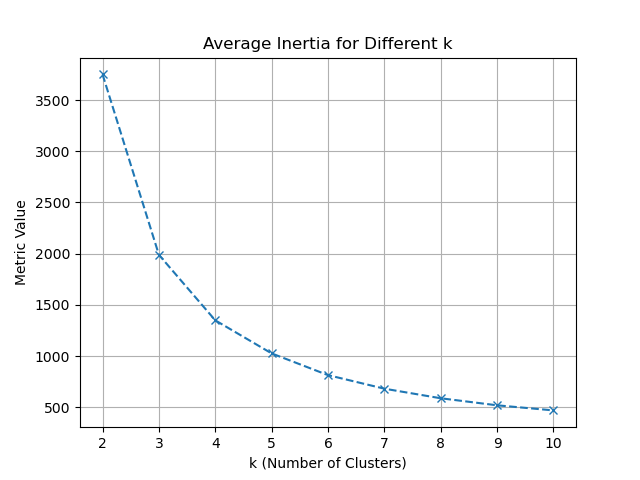
\includegraphics[width=0.8\textwidth]{Pictures/Average Inertia}
\caption{Graph for Average Inertia for K}
\label{fig:1}
\end{figure}

\begin{figure}[ht]
\centering
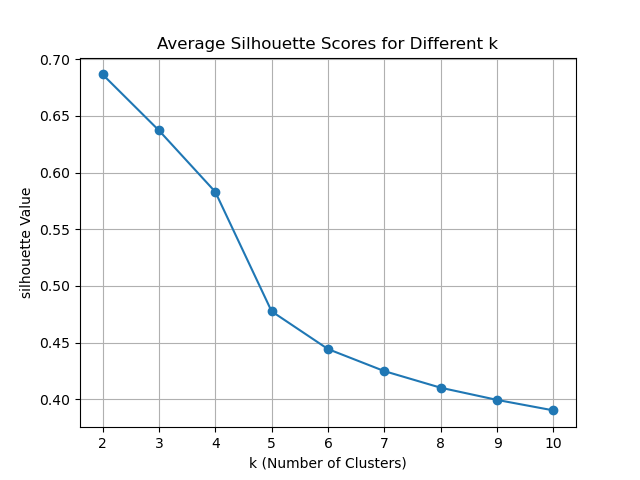
\includegraphics[width=0.8\textwidth]{Pictures/Average Silhouette Score}
\caption{Graph for Average Silhouette scores for K}
\label{fig:2}
\end{figure}

\begin{figure}[ht]
\centering
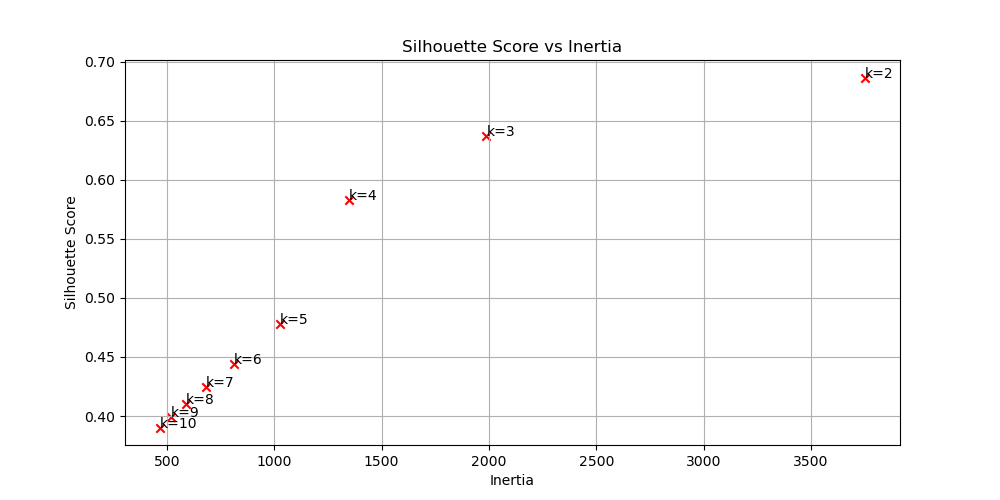
\includegraphics[width=0.5\textwidth]{Pictures/Silhouette score vs Inertia}
\caption{Graph for the Silhouette Score vs. Inertia}
\label{fig:3}
\end{figure}

\begin{figure}[ht]
\centering
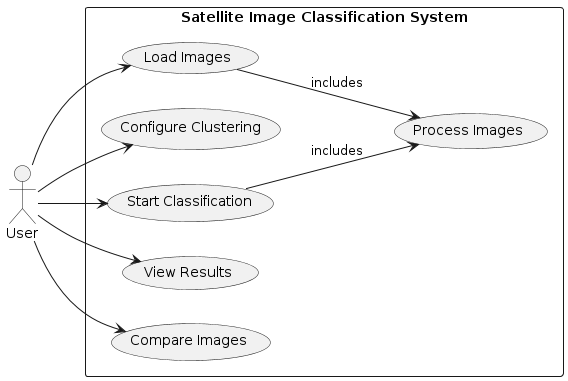
\includegraphics[width=0.4\textwidth]{Pictures/Use case Diagram}
\caption{Use case Diagram}
\label{fig:5}
\end{figure}

\begin{figure}[ht]
\centering
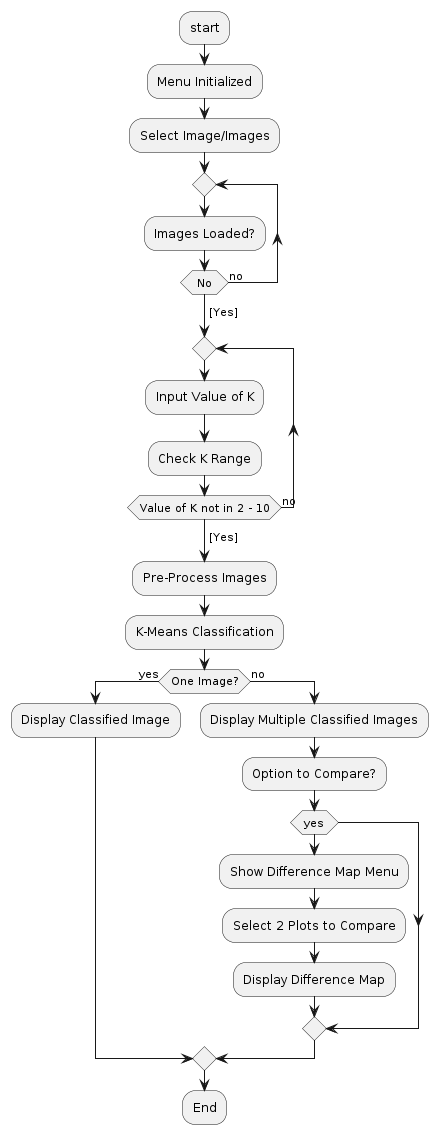
\includegraphics[width=0.4\textwidth]{Pictures/Program Flowchart}
\caption{}
\label{fig:6}
\end{figure}


\section{tables}\label{sec:tables}

\begin{table}[ht]
\centering
\caption{Feature List}
\begin{tabular}{|c|p{3cm}|p{4cm}|p{4cm}|}
\hline
\textbf{Feature Number} & \textbf{Feature Name} & \textbf{Feature Description} & \textbf{Acceptance Test} \\ \hline
1 & Load Satellite Imagery & Users should be able to upload and store satellite images & Users can upload images in supported formats (e.g., JPG). The system confirms successful uploads  \\ \hline
2 & View Images & Users should be able to view and manage their uploaded satellite images & All uploaded images are displayed in the user dashboard with options to zoom and pan\\ \hline
3 & Configure classification & Users should be able to configure parameters for classification & Users can select and set parameters such as number of clusters\\ \hline
4 & Start Classification & Users should be able to initiate the classification process on selected images & Classification process starts, and the system displays processing status.\\ \hline
5 & View Classification Results & Users should be able to view and analyze the results of image classifications & Results, including cluster maps and metrics are displayed for user analysis. \\ \hline
6 & Change Detection & Users should be able to compare classification results over time & comparison interface allows user to view a diff map of the two areas with the differences highLighted\\ \hline
\end{tabular}\label{tab:1}
\end{table}


\begin{table}[ht]
\centering
\caption{Test Descriptions}
\begin{tabular}{|c|p{3cm}|p{5cm}|c|}
\hline
\textbf{Test Number} & \textbf{Test Name} & \textbf{Test Description} & \textbf{Pass or Fail} \\ \hline
1 & File Format Compatibility Test & Upload a file which is jpg or png & Pass \\ \hline
2 & File Size and Resolution Test & Upload a very large Image & Pass \\ \hline
3 & Corrupted File Handling & Upload a corrupted image file & Fail \\ \hline
4 & Multi-file Upload Test & Upload multiple Files at once & Pass \\ \hline
6 & Upload Limits and Restrictions & Upload as many files as You can, should be able to & Pass \\ \hline
\hline
\end{tabular}\label{tab:2}
\end{table}

\fancypagestyle{plain}{%
   \fancyhead{} %[C]{Annotated Bibliography}
   \fancyfoot[C]{{\thepage} of \pageref{LastPage}} % except the center
   \renewcommand{\headrulewidth}{0pt}
   \renewcommand{\footrulewidth}{0pt}
}

%TC:endignore

\end{document}
